% -*- TeX-master: "../all_the_notes.tex" -*-

\section{Fabrication}
\label{sec:fabrication}

\textit{Fabrication is not  an easy thing, and yet it  can be completed
  in the space of a single week}

\subsection{No Category}
\label{sec:no-category}

\begin{framed}\noindent
  \begin{itemize}
  \item Always ground the qubits directly - never through a capacitor;
  \end{itemize}
\end{framed}

\subsection{Macroscopic parameters}\label{sec:size-parameters}
\begin{figure}[ht]
  \centering         \includegraphics[height=4cm]{fabrication_cassette}
  \includegraphics[height=4cm]{qubit_chip_annotated}
  \caption{\small   Big  markers   are   the   P,Q  markers   described
    below.\label{fig:qubit_chip}}
\end{figure}
\begin{enumerate}
\item \textbf{Sample chips} are mounted in a cassette with windows. The
  available sizes are:

  \begin{itemize}
  \item \iunit{18}{mm} x \iunit{18}{mm};
  \item \iunit{13}{mm} x \iunit{13}{mm};
  \item \iunit{8}{mm} x \iunit{8}{mm}.
  \end{itemize}

  \noindent \red{\textbf{The  chip must be  larger than this  window in
      order to be fixed in place.}}

\item \textbf{Qubit  chip}: \iunit{5}{mm} x \iunit{3}{mm}.   This means
  that a \iunit{18}{mm} chip will fit $ 3\times7 $ of them.

\item  \textbf{Transmission  line}:  is   characterized  by  width  and
  separation  with the  ground planes.   \red{\textbf{This defines  the
      impedance of the line, which must be 50$\Omega$}}.

  \begin{itemize}
  \item  \textbf{Narrow:}  Width  =  \iunit{20}{$\mu$m},  Separation  =
    \iunit{12}{$\mu$m};
  \item  \textbf{Wide:}   Width  =  \iunit{55}{$\mu$m},   Separation  =
    \iunit{30}{$\mu$m};
  \item  The  width  determines  the   speed  of  propagation  -  wider
    $ \equiv $ greater speed and higher frequencies.
  \end{itemize}

  \begin{center}
    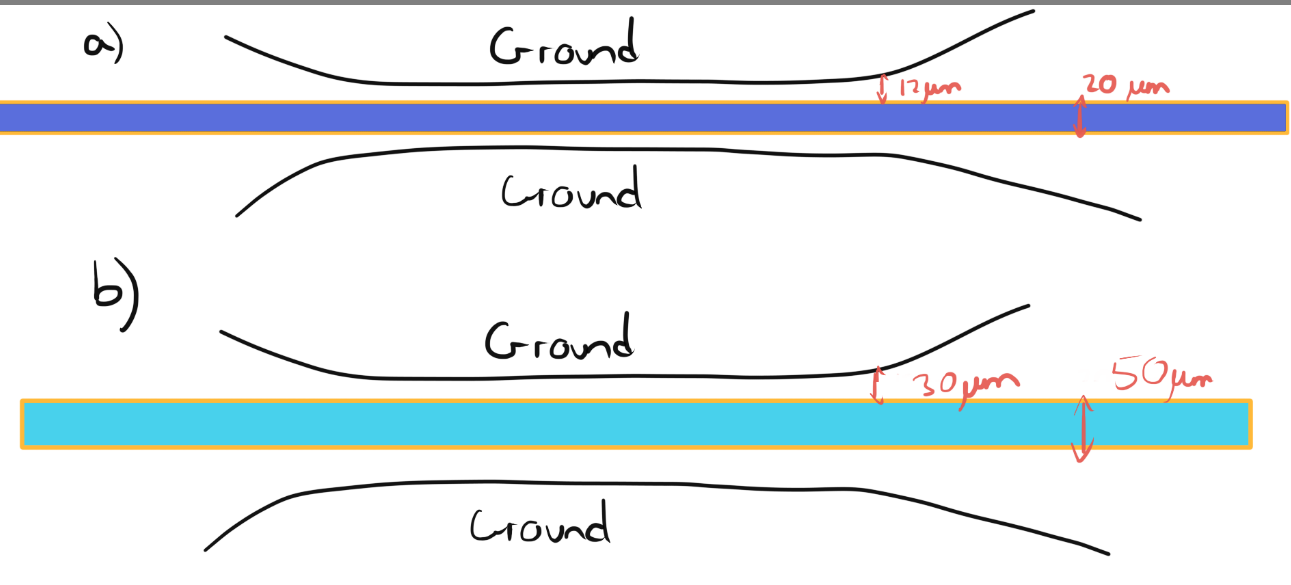
\includegraphics[height=3cm]{fab_transmission_line}
  \end{center}
\end{enumerate}

\subsection{Resonators}
\label{sec:resonators}

\noindent Resonators designed by Rais come in two lengths:
\begin{itemize}
\item \iunit{400}{$\mu$m};
\item \iunit{200}{$\mu$m}.
\end{itemize}

\noindent The frequency of a resonator is given by:

\begin{equation}
  \label{eq:fabrication_groupSpeed}
  \begin{aligned}
    & f j= \frac{v}{L_{r}}\\
    & \begin{cases}
      v = \frac{1}{\sqrt{L*C}}\\
      L = \text{ inductance per unit length}\\
      C = \text{ capacitance per unit length}\\
      L_{r} = \text{ length of resonator}
    \end{cases}
  \end{aligned}
\end{equation}

\noindent

\newpage\subsection{Materials parameters}
\label{sec:materials-parameters}

\begin{framed}\noindent
  In a charge qubit, the only  part that needs to be superconducting is
  the    JJ     superconducting-insulator-superconducting    structure.
  \red{\textbf{All other components  can be made from  normal metal, as
      there is no persistent current.}}
\end{framed}

\subsubsection{Transition temperatures}
\label{sec:trans-temp}
\begin{itemize}
\item NbN\hfill \iunit{4.5}{K};
\item Al \hfill \iunit{1.3}{K};
\item Ti \hfill \iunit{0.63}{K}.
\end{itemize}

\newpage\subsection{Deposition}
\label{sec:deposition}


\begin{itemize}
\item \textbf{Ground planes and  bonding contacts:} Ti (\iunit{10}{nm})
  - Au (\iunit{80}{nm})
\item \textbf{Aluminum JJ:}
  \begin{itemize}
  \item Copolymer 13\% \hfill \red{T = 600nm};
  \item  Either ZEP520a:Anisol  1:2  or ARP6200\  4\%  \hfill \red{t  =
      100nm};
  \item \red{\textbf{The undercut is 150\,nm}};
  \item Angle evaporation leads to:
    \begin{itemize}
    \item Shift in the pattern by $ T\tan(\alpha) $;
    \item Shortening of the pattern by $ t\tan(\alpha) $.
    \end{itemize}
  \item Meaning that  in order to get an overlap  between \red{red} and
    \gold{yellow} we need to shift the deposition holes;
  \end{itemize}
  \begin{figure}[h]
    \centering \includegraphics[height=8cm]{fabrication_angle}
    \caption{\small    Angle   $\alpha$    shifts   the    pattern   by
      $ T\tan(\alpha) $  and shortens it by $  t\tan(\alpha).$ Thus the
      pattern needs  to be made longer  and shifted to get  the desired
      structure. \label{fig:fabrication_angle}}
  \end{figure}
  \begin{itemize}
  \item Shift the bottom layer and top layer in opposite directions by
    \begin{equation}
      \label{eq:jj_overlap}
      \text{Shift} = T\tan(\alpha).
    \end{equation}
  \item  Elongate  the windows  \red{\textbf{on  the  inner sides}}  by
    \hfill \textbf{NO NEED TO DO THIS}
    \begin{equation}
      \label{eq:jj_elongate}
      \text{Elongate} = t\tan(\alpha),
    \end{equation}
  \end{itemize}
\end{itemize}
\begin{framed}\noindent
  For T  = \iunit{600}{nm} and  t = \iunit{100}{nm} and  12$^o$: \hfill
  \red{Shift = \iunit{150}{nm}};

  \noindent For T = \iunit{600}{nm}  and t = \iunit{100}{nm} and 9$^o$:
  \hfill \red{Shift = \iunit{110}{nm}};

  The separation between neighbouring holes for the resist to be stable
  is 100\,nm.



\begin{center}
  \red{After the first deposition the mask gets smaller, so avoid vertical symmetry} \\
\end{center}
\end{framed}

\subsubsection{Perpendicular deposition}
\label{sec:perp-depos}

A  better deposition  is  the  one that  was  proposed  by Rais,  where
deposition is done at 0 and 30 degrees.
\begin{figure}[h]
  \centering \inkfig{15cm}{0and30}
  \caption{\small  Perpendicular deposition  followed  by 30$^o$  angle
    deposition     will     remove     the    ``shadow''     of     the
    tbar.\label{fig:0and30}}
\end{figure}


\subsection{Coupling-capacitance}
\label{sec:coupling-capacitance}

\begin{framed}\noindent
  \begin{itemize}
  \item   Separation  of   elements   should  be   of   the  order   of
    \iunit{2}{$\mu$m};
  \item  \red{\textbf{Each  \iunit{10}{$\mu$m} of  parallel  structures
        adds on \iunit{1}{fF} of capacitance.}}
  \end{itemize}

   \begin{center}
     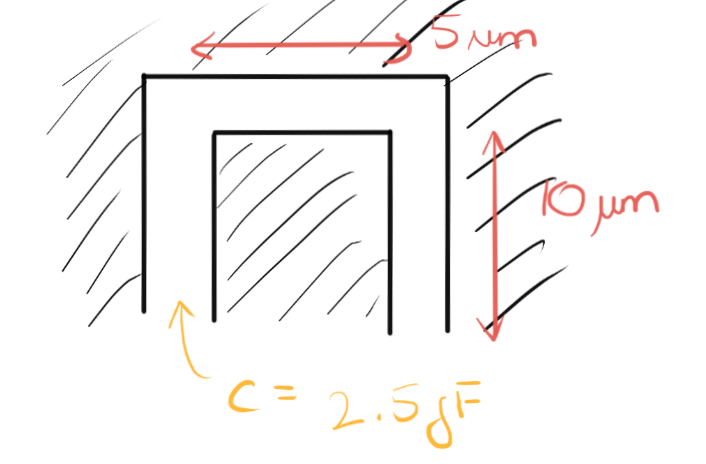
\includegraphics[height=4cm]{fab_capacitance} {\small  Think of it
       as counting the length of  the meander between structures.  Each
       \iunit{10}{$\mu$m}           of            length           adds
       \iunit{1}{pA}.\label{fig:example-image-c}}
   \end{center}
 \end{framed}


 \subsection{Josephson parameters}
 \label{sec:josephson-parameters}
 \begin{equation}
   \label{eq:fabrication_jj_1}
   \begin{aligned}
     & \red{E = E_J(1-\cos(\phi))} \\
     & \begin{cases}
       E_J = \frac{\Phi_0I_c}{2\pi}\\
       I_cR_n =  \frac{\pi\Delta(0)}{2e} \qquad  \text{critical current
         from BCS theory.}
     \end{cases}
   \end{aligned}
 \end{equation}

 \noindent A  typical JJ  will have  an area  of say  \iunit{100 \times
   200}{nm}$^{2}$

 \begin{framed}\noindent
   \begin{equation}\label{eq:fabrication_jj_2}
     \begin{aligned}
       & E_J = \frac{R_q}{R_n/N_{sq}}\frac{\Delta(0)}{2}\\
       & \begin{cases}
         R_n = 18.4\,\text{k}\Omega \qquad \text{sheet resistance of 100 } \times 100\,\text{nm}^{2}\\
         R_q = \frac{h}{(2e)^2}
       \end{cases}
     \end{aligned}
   \end{equation}
   \noindent The wider the JJ is in  squares, $ N_{sq} $, the lower the
   resistance   of  the   junction.   The   calibration  graph   for  a
   $ 200 \times \iunit{800}{nm}^2 $ junctions is shown below:

   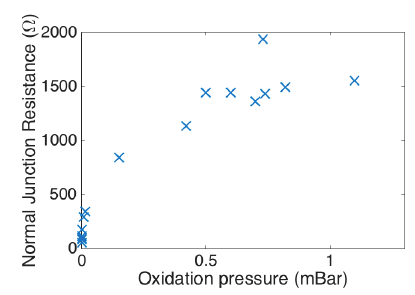
\includegraphics[height=4cm]{oxidation}

   \red{JJ resistance increases by $ \sim  10\% $ as one goes from room
     to cryogenic temperatures.}
 \end{framed}

 % The resistances go as follows:

 % \begin{table}[h]
 %   \centering
 %   \begin{tabular}{|c|c|c|}
 %     \textbf{Resistance}    & \textbf{Symmetrical JJ} & \textbf{Straddled}\\
 %     \iunit{1}{k$\Omega$} & 4838 & 2710 \\

 %   \end{tabular}
 %   \caption{Resistance of JJ}
 %   \label{tab:resistances_jj}
 % \end{table}


 \subsection{Capacitance parameters}
 \label{sec:capac-param}

\begin{equation}\label{eqn:sim_1}
  E_c = \frac{(2e)^2}{2C},
\end{equation}

\noindent  we need  the capacitance  of the  JJ. We  can treat  the two
overlapping parts of the JJ acting a parallel plate capacitor with

\begin{framed}\noindent
  \begin{equation}\label{key}
    C = \frac{\varepsilon\varepsilon_0A}{d},
  \end{equation}

  \noindent   with   the   permittivity  for   Aluminum   oxide   being
  $ \varepsilon \approx 10 $ and thickness $ d \approx \iunit{2}{nm} $.
  This  give s  a  junction 200  $ \times  $  800\,nm$^{2}$ a  charging
  frequency of $ E_c/\hbar \approx\iunit{19}{GHz} $.
\end{framed}

\newpage\subsection{Summary}
\label{sec:summary}

\hspace{-3cm}\begin{table}[h] \centering
  \begin{tabular}{|c|c|p{6cm}|c|}
    \hline\textbf{Energy} &  & \textbf{Variable  parameter} &
                                                              \textbf{Energy ($ N_{sq}=10, N_{NbN} = 5$)}\\\hline
    $ E_J $ & $ \frac{R_q}{R_{\square}/N_{sq}}\frac{\Delta(0)}{2} $ & $ R_q = \frac{h}{(2e)^2} = 6.484\,\text{k}\Omega,\newline \Delta = 1.73*(k_b\times 1.3\,\text{K}) = 3.1\times10^{-23}, \newline R_\square = \iunit{18.4}{k}\Omega $ & \iunit{77.5}{GHz}\\\hline

    $ E_C $ & $ \frac{(2e)^2}{2CN_{sq}} $ & $ \varepsilon = 10, d = \iunit{2}{nm}, \newline A = 100\times\iunit{100}{nm}^2, \newline C = \frac{\varepsilon\varepsilon_0A}{d} = \iunit{0.5}{fF} $ & \iunit{17.4}{GHz}\\\hline

    $       E_L       $       &        $       \frac{\Phi_0^2}{(2\pi)^22LN_{NbN}}       $       &
                                                                                                  $  \Phi_0 =  2\times10^{-15}\,\text{Wb}, \newline  L =
                                                                                                  \iunit{1.5}{nH}
                                                                                                  $
                                                                                                  per
                                                                                                  NbN
                                                                                                  square
                                                            &
                                                              \iunit{16.2}{GHz}\\\hline
  \end{tabular}
\end{table}


\newpage \subsection{Autocad-Beamer Design}
\label{sec:autocad-design}

\begin{itemize}
\item All shapes \textbf{must} be polylines.  They must be joined up in
  a single line, or they wont work;
\item Units are in microns;
\item \red{\textbf{Place small markers in the corners of the pattern so
      that centering is correct}};
\item Once design  is finished, \texttt{select all \ira  Purge \ira All
    \ira type "none*" \ira Yes to all};

\item \red{\textbf{Decide  on the  P, Q  markers that  will be  used to
      align the chip - note down their chip coordinates}}
\end{itemize}

\newpage\subsection{Typical exposure}
\label{sec:typic-expos-param}
\begin{itemize}
\item Depending  on the current you'd  like to use, you  have to choose
  between:
  \begin{itemize}
  \item High  Throughput: EOS  mode 3,  100 keV, lens  4, from  2nA and
    above
  \item High Resolution: EOS mode 6, 100 keV, lens 5, 100-400 pA.
  \end{itemize}
\item \iunit{100}{nA} for the bulky regions;
\item \textbf{Reading markers:}
  \begin{enumerate}
  \item Select window to work with: A, B, C or D;
  \item Find  global markers P,Q that  are usually on the  periphery of
    the chip (green)
  \item For each chip define a chip mark (blue) e.g. 490,490;
  \item Specify  the center the  central chip (-3500,2500) so  that the
    chip pattern is tied to the global markers.
  \end{enumerate}
  \begin{figure}[h]
    \centering \includegraphics[height=8cm]{jeol_layout}
    \caption{\small Red  is the  measured values of  the P,  Q markers.
      Green   is    the   designed   positions   that    are   set   as
      targets. \label{fig:jeol_layout}}
  \end{figure}
\end{itemize}
